
%\documentclass[justified, marginals=raggedouter]{tufte-handout}
\documentclass[justified, marginals=justified]{tufte-handout}

% Adding a few custom packages
\usepackage{tcolorbox}
\usepackage{lipsum}
\usepackage{bm,upgreek}

\usepackage{amssymb}
% let's you use trinalgeq


\newenvironment{rcases}
{\left.\begin{aligned}}
	{\end{aligned}\right\rbrace}
% let's you use right curly braces next to array

\usepackage{subfig}
% Example environment
\usepackage{amsthm}
\theoremstyle{definition}
\newtheorem{exmp}{Example}

% The default minimumo amount of space between \marginnotes is 10 pt.
\setlength\marginparpush{1cm}

\title{6.864 Advanced Natural Language Processing\thanks{Instructors: Prof. Regina Barzilay, and Prof. Tommi Jaakkola.\\ TAs: Franck Dernoncourt, Karthik Rajagopal Narasimhan, Tianheng Wang. \\ Scribes: Dongyoung Kim.}}

\author[Lecture 4: EM Algorithm and Topic Model]{Lecture 4: EM Algorithm and Topic Model}

\date{24 September 2015} % without \date command, current date is supplied

%\geometry{showframe} % display margins for debugging page layout

\usepackage{graphicx} % allow embedded images
  \setkeys{Gin}{width=\linewidth,totalheight=\textheight,keepaspectratio}
  \graphicspath{{graphics/}} % set of paths to search for images
\usepackage{amsmath}  % extended mathematics
\usepackage{booktabs} % book-quality tables
\usepackage{units}    % non-stacked fractions and better unit spacing
\usepackage{multicol} % multiple column layout facilities
\usepackage{lipsum}   % filler text
\usepackage{fancyvrb} % extended verbatim environments
  \fvset{fontsize=\normalsize}% default font size for fancy-verbatim environments

% Standardize command font styles and environments
\newcommand{\doccmd}[1]{\texttt{\textbackslash#1}}% command name -- adds backslash automatically
\newcommand{\docopt}[1]{\ensuremath{\langle}\textrm{\textit{#1}}\ensuremath{\rangle}}% optional command argument
\newcommand{\docarg}[1]{\textrm{\textit{#1}}}% (required) command argument
\newcommand{\docenv}[1]{\textsf{#1}}% environment name
\newcommand{\docpkg}[1]{\texttt{#1}}% package name
\newcommand{\doccls}[1]{\texttt{#1}}% document class name
\newcommand{\docclsopt}[1]{\texttt{#1}}% document class option name
\newenvironment{docspec}{\begin{quote}\noindent}{\end{quote}}% command specification environment

\begin{document}

\maketitle% this prints the handout title, author, and date

Earlier, we saw cases where the full data was observable and we could apply a straightforward maximum-likelihood estimator for the parameters. In Lecture 4, we introduce a Hidden Variable Model where data is partially observable. Then, we provide basic intuitions for the EM algorithm which can be used to optimize the likelihood on such Hidden Variable Models. We explore further by demonstrating the EM algorithm on a toy example with biased coins. Later, we connect our concept to more relevant topics in NLP such as topic modeling.  

\section{Hidden Variable Models}\label{sec:hidden-variable-models}

\subsection{Motivation}\label{sec:motivation}

Hidden Variable Models are very common in NLP applications. To gain intuition, see the following examples. 

\begin{enumerate}
	\item \textit{Topic Model}: Consider the following traditional unigram model. Suppose document $D$ is comprised of $N$ words such that $D=\{w_1, w_2, ..., w_N\}$. Given a unigram distribution $p(w_i)$, the log-likelihood of any document will be given by the same form 
	\begin{align*}
		\log p(D) = \sum_{i=1}^{N} \log p(w_i)
	\end{align*}
	However in practice, each documents are different and therefore we may want to use different distributions over the words depending on the context. 	
	 This idea can be easily implemented in Topic Models. A topic is denoted by $z$ where $z\in\mathcal{Z}$, and $\mathcal{Z}$ is our pre-defined universe of topics of $k$ dimension. Each word $w_i$ is sampled from a corresponding topic $z_i$. 
	 
	 The problem in Topic Models arise from the fact that the topic information is not provided in the training corpus. If the entire data had been observed, we could simply estimate the conditional distribution as the empirical count,
	\begin{align}
	\hat{p}(w|z) = \dfrac{count(w,z)}{count(z)}
	\end{align}
	
		\begin{marginfigure}[-3cm]%
			\centering
			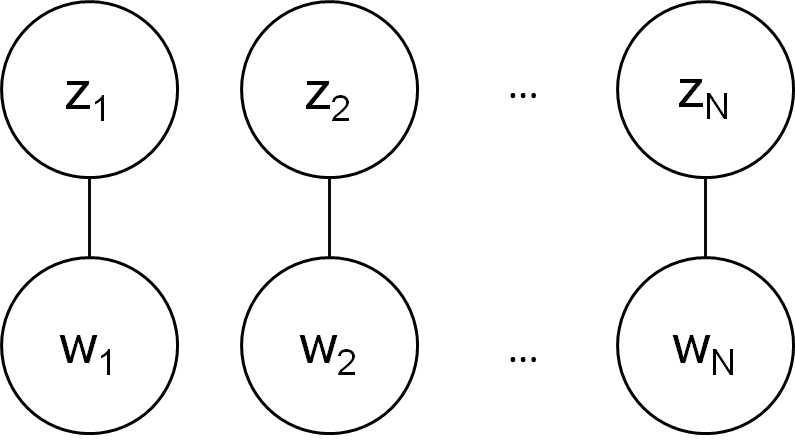
\includegraphics[width=4cm]{topic-model-unigram.png}
			\caption{Topic model is where each word is associated with a conditional topic. For example, it is more likely to observe word $w_i="Cat"$ if the topic is $z_i="Pets"$.}
			\label{fig:topic-model-unigram}
		\end{marginfigure}
	
	However, such straightforward approach seen in (1) is no longer applicable if the variables $z_i$ are hidden. Since it is unlikely to have each word in a document explicitly tagged with its related topics, topic models naturally arise as Hidden Variable Models.
	
	\item \textit{Machine Translation Alignment}: 
	In Machine Translation, one is given two sentences in different languages with the same meaning. As seen in Figure~\ref{fig:machine-translation-alignment}, when the word \textit{"I"} is paired together many times with the corresponding Korean word, then it is probably a good indicator that \textit{"I"} should be translated to that word. Therefore, the first step in Machine Translation is to align corresponding translations. However, the alignments are not explicitly given in real life applications and should be treated as hidden variables one has to estimate. 
		\begin{marginfigure}[-3cm]%
			\centering
			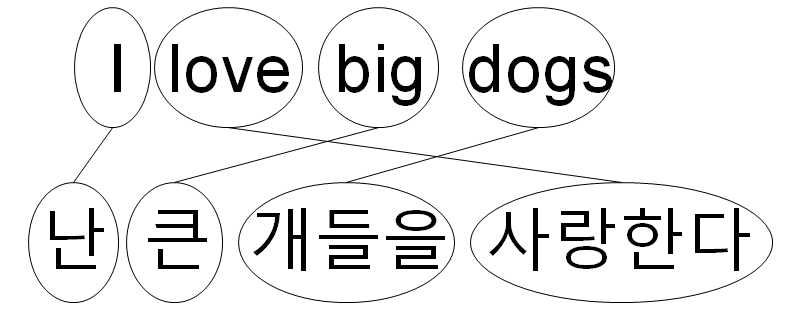
\includegraphics[width=4cm]{machine-translation-alignment.png}
			\caption{In machine translation, each word from one language has a hidden alignment to its counterpart.}
			\label{fig:machine-translation-alignment}
		\end{marginfigure}	

	\item \textit{Part-of-Speech Tagging}: Part-of-speech tagging, which will be covered in the next lecture, matches each word in a sentence with its part of speech in English. For the example in Figure~\ref{fig:part-of-speech}, \textit{"I"} is tagged with \textit{"pronoun"}, \textit{"love"} with \textit{"verb"}, \textit{"big"} with \textit{"adjective"}, and \textit{"dogs"} with \textit{"noun"}. When the full observed data observable, one can apply a supervised learning algorithm. However when the parts of speech are not observed, then they are treated as hidden variables. 
		\begin{marginfigure}[-3cm]%
			\centering
			
\includegraphics[width=3.5cm]{part-of-speech.png}
			\caption{Each word is associated with a hidden part-of-speech in English.}
			\label{fig:part-of-speech}
		\end{marginfigure}	
\end{enumerate}

\subsection{Observed Case vs. Unobserved Case}\label{sec:observed-case-vs-unobserved-case}

In previous lectures we looked at models where the full data was observed. We use 
\begin{align*}
D = \{(x_1, y_1), (x_2, y_2), ..., (x_N, y_N)\}
\end{align*}

\noindent to denote the given dataset in such cases, which is represented as a list of sampled tuples. Each data point $(x, y)$ is independently sampled from some distribution $p_{\text{X,Y}}(x,y)$ parameterized by $\theta$. The objective function we are trying to maximize is given by the following
\begin{align}
\label{eq:observed}\theta^{*} = \underset{\theta}{\operatorname{argmax}}\sum_{i=1}^{N}\log{p_{\text{X,Y}}(x_i, y_i|\theta) }
\end{align}

Now, let's look at the unobserved case where $\textbf{y}$ is unseen. In other words, $\textbf{x}$ is the observed variable and $\textbf{y}$ is the hidden variable. In this case, the observed data is given by
\begin{align*}
D = \{x_1, x_2, ..., x_N\}
\end{align*}
In this case, we replace the objective function with the log-likelihood of the \textit{partially observed data}, which is
\begin{align}
\theta^{*} &= \underset{\theta}{\operatorname{argmax}}\sum_{i=1}^{N}\log{p_{\text{X}}(x_i|\theta) } \nonumber \\
\label{eq:unobserved}&= \underset{\theta}{\operatorname{argmax}}\sum_{i=1}^{N}\log\sum_{y\in \mathcal{Y}}p_{\text{X,Y}}(x_i, y|\theta)
\end{align} 

\noindent where the second equality is due to marginalization over $y$ over $p_{ \text{X,Y} }(x,y)$. The key point is to note that the criteria for the observed case and the unobserved case is different, and we should use a different objective function when we are trying to optimize for the parameter $\theta$. In the following sections we will demonstrate how the EM algorithm finds the optimum parameter for (\ref{eq:unobserved}).

Before we see how the EM algorithm can optimize (\ref{eq:unobserved}), let's first how we can compute the solution for (\ref{eq:observed}) through a simple example. 

\begin{exmp}\label{dog-cat-example}
	Assume a simple unigram model where there are two words in the universe such that $V = \{\text{"dog"}, \text{"cat"}\}$. There is one free parameter given by
	\begin{align*}
	\theta &= p(\text{"dog"}) \\
	1-\theta &= p(\text{"cat"})
	\end{align*}
	Given document $D=\{w_1, w_2, ..., w_N\},$ the log-likelihood of the document is given by
	\begin{align*}
	l(D|theta) &\triangleq  \log p(D|\theta) \\
	&= \log( \theta^{d}(1-\theta)^{c} ) \\
	&= d\cdot \log \theta + c\cdot \log (1-\theta)
	\end{align*}
	
	Where $d$ is a constant equal to the number of occurrence of "dog" in the document, and $c$ is equal to that of "cat". To compute $\theta^*$, we take the partial derivative of the log-likelihood with respect to $\theta$ and set it to zero. 
	\begin{align*}
	\dfrac{\partial l(D|theta)}{\partial \theta}&=\frac{d}{\theta^*}-\frac{c}{1-\theta^*} \\
	&= 0
	\end{align*}
	Multiplying $\theta^*(1-\theta^*)$ to both sides,
	\begin{align*}
	d(1-\theta^*) - c\theta^* &= 0 \\
	d - d\theta^* -c\theta^* &= 0 \\
	(d+c)\theta^* &= d \\
	\llap{$\rightarrow$\hspace{50pt}} \theta^* &= \frac{d}{d+c}
	\end{align*}
	We can easily derive that the Maximum Likelihood Estimator is given by the fraction of the empirical counts.
	
\end{exmp}

\section{EM Algorithm}\label{sec:em-algorithm}
\begin{exmp}\label{em-example}

We will now set up a simple example to walk through how the EM algorithm works. Suppose we have a card and two different coins, where all probabilities are biased. We will take the following steps to sample a sequence of coin flips.
\begin{enumerate}
	\item Flip the card, which either returns side \textit{A} or side \textit{B}.
	\item If \textit{A} was drawn from step 1, toss coin \text{1} three times. Otherwise if \textit{B} was drawn, toss coin 2 three times. 
	\item repeat steps 1-2
\end{enumerate}

Expressing this more formally, $y$ represents the side of the card and $x$ represents the outcome of three consecutive coin tosses. $H$ and $T$ denotes the head and tail of a coin, respectively. 
\begin{align*}
y \in \mathcal{Y} &= \{A, B\} \\*
x \in \mathcal{X} &= \{HHH, HTH, ..., TTT\}
\end{align*}
\indent Furthermore, let us assume that we did not see the card values $y$, and we could only observe the sequence of the coin flips $x$. Since the data is partially observed, this example is an instance of a Hidden Variable Model.

There are three free parameters in this setup, given by $\bm\uptheta = \{\alpha, p_A, p_B \}$. The parameters are described as follows
\begin{align*}
\alpha &= p(Card = A) \\*
p_A &= p(Coin 1 = H) \\*
p_B &= p(Coin 2 = H) 
\end{align*}
It is easy to see that
\begin{align*}
p(x,y|\bm\uptheta) &= p(y|\bm\uptheta)p(x|y,\bm\uptheta) \\*
p(y|\bm\uptheta) &= \left\{ 
	\begin{array}{l l}
		\alpha & \quad \text{if $y = A$}\\
		1-\alpha & \quad \text{if $y = B	$}
	\end{array} \right.\\*
p(x|y,\bm\uptheta) &= \left\{ 
	\begin{array}{l l}
		p_A^{h(x)}(1-p_A)^{t(x)} & \quad \text{if $y = A$}\\
		p_B^{h(x)}(1-p_B)^{t(x)} & \quad \text{if $y = B	$}
	\end{array} \right.
\end{align*}

Where we define $h(x)$ to be a function that is equal to the number of heads in sample $x$, and $t(x)$ to be the number of tails. For example, if $x_0 = {HHT}$, then $h(x_0) = 2$ and $t(x_0) = 1$.  

\end{exmp}

\subsection{Observed Case}\label{sec:observed-case}
Let's go back on our assumption that the card values $\mathbf{y}$ were hidden, and say the card flips and the coin tosses were entirely observable. Each card flip is associated with three coin tosses. Suppose after three iterations, the observed data was given as follows
\begin{align*}
D = \{(A, HHH), (A, HHH), (B, TTT)\}
\end{align*}

where $(y,x) = (A, HHH)$ denotes that the observed card flip was $A$, followed by three heads. Earlier in Example \ref{dog-cat-example}, we have seen that applying partial derivative to the log-likelihood given in \eqref{eq:observed}, the MLE parameters are simply given by the empirical counts. Using this fact for granted, the parameter values for these specific samples are given by

\begin{equation*}
\begin{rcases}
\alpha^{*} &= \dfrac{\text{count(A)}}{3}=\dfrac{2}{3} \\
p_A^{*} &= \dfrac{ \text{count}(A,H)} { \text{count}(A, H)+\text{count}(A, T) } = \dfrac{6}{6} \\
p_B^{*} &= \dfrac{ \text{count}(B,H)} { \text{count}(B, H)+\text{count}(B, T) } = \dfrac{0}{3}
\end{rcases}
\text{\quad MLE parameters}
\end{equation*}

Shortly we will see that this analytic solution has a very similar form to the solution for each iteration in the EM algorithm, which is covered in the next section. 

\subsection{Unobserved Case}\label{sec:unobserved-case}

Continuing with the problem setup in Example \ref{em-example}, suppose the card flips are no longer observable. In other words, we will treat the card flip $y$ as a hidden variable. Consider the following sample data
\begin{align*}
D = \{HHH, HHH, TTT\} = \textbf{x}
\end{align*}

Let us make an initial guess on the parameter values. Assign arbitrary prior values such that 
\begin{align}
\label{priors}
\alpha^{(0)} = 0.1,\quad p_A^{(0)}=0.8,\quad p_B^{(0)}=0.5\quad
\end{align}
The initial guess in (\ref{priors}) is denoted with a superscript 0 to mark that this is the belief of the parameters at time 0. We will see how the belief is updated over each iteration of the EM algorithm. 

For each $x_i $ in the dataset, we compute $p_{\text{Y|X}, \bm\uptheta}(y|x_i, \bm{\uptheta}^{(0)})$ over all possible values of $y \in \mathcal{Y} = \{A, B\}$.  For example, for our  For $x_1 = HHH$ in the given example dataset,
\vspace{3mm} \\
\begin{math}
\-\hspace{0ex} p(y_1=A|x_1=HHH, \bm{\uptheta}^{(0)}) \\
\-\hspace{0ex} = \dfrac { p(x_1=HHH, y_1=A | \bm{\uptheta}^{(0)}) }
{p(x_1=HHH, y_1=A | \bm{\uptheta}^{(0)})+p(x_1=HHH, y_1=B | \bm{\uptheta}^{(0)})} \\*
\-\hspace{0ex} = \dfrac{ \alpha p_A^3 }{ \alpha p_A^3 + (1-\alpha) p_B^3 } \vspace{2mm} \\*
\-\hspace{0ex} = \dfrac{0.1\times0.8^3}{0.1\times0.8^3 + (1-0.1)\times 0.5^3} \approx 0.3  \\* 
\\*
\\*
\-\hspace{0ex} p(y_1=B|x_1=HHH, \bm{\uptheta}^{(0)}) \\  %equation2
\-\hspace{0ex} = \dfrac{ p(x_1=HHH, y_1=B | \bm{\uptheta}^{(0)}) }
{p(x_1=HHH, y_1=A | \bm{\uptheta}^{(0)})+p(x_1=HHH, y_1=B | \bm{\uptheta}^{(0)})} \\*
\-\hspace{0ex} = \dfrac{ (1-\alpha) p_B^3 }{ \alpha p_A^3 + (1-\alpha) p_B^3 } \vspace{2mm} \\*
\-\hspace{0ex} = \dfrac{(1-0.1)\times0.5^3}{0.1\times0.8^3 + (1-0.1)\times 0.5^3} \approx 0.7
\end{math}
\vspace{3mm} \\
Recall from the previous section that in the fully observed case, each $x_i$ was explicitly associated with a \textit{single} count of either $y_i=A$ or $y_i=B$. In the unobserved case, we assume that each $x_i$ is associated with \textit{fractional counts} over all possible values of $y_i$, to which we assign the \textit{expected count} of $y_i$ given $x_i$ and our prior knowledge of $\bm{\uptheta}$.

\begin{table}[h]
	\centering
	\subfloat[$y$ is observed]{
		\begin{tabular}{ccc}
			\toprule
			$x_i$ & $y_i$ & empirical count \\
			\midrule
			HHH & A & 1 \\
			 &  &  \\
			HHH & A & 1 \\
			 &  &  \\
			TTT & B & 1 \\
			 &  &  \\
			\bottomrule
		\end{tabular}
	}
	\quad
	\subfloat[$y$ is unobserved]{
		\begin{tabular}{ccc}
			\toprule
			$x_i$ & $y_i$ & fractional count \\
			\midrule
			HHH & A & 0.3 \\
			  & B & 0.7 \\
			HHH & A & 0.3 \\
			& B & 0.7 \\
			TTT & A & 0.5 \\
			& B & 0.5 \\
			\bottomrule
		\end{tabular}
	}
	\caption{In the fully observed case (a), a single value of $y$ (which is the observed value itself) is associated with each $i^{\text{th}}$ data sample. In the unobserved case (b), we assume that a entire list over the alphabet $\mathcal{Y}$, is associated with $x_i$. Each element in the spectrum is assigned a weight, or the \textit{fractional count}, which corresponds to the expected value of $y$ given $x_i$. The fractional count can also be understood as the confidence in the sample ($x_i, y_i$) given a prior belief over the parameters. }
\end{table}

\vspace{3ex}
Hereafter the remaining steps are almost identical to the MLE maximization of the parameters. Again we will derive our distribution by counting, but since the actual counts are no longer available, we will count the fractional counts instead. The parameters for the next iteration, or time 1, will be computed as follows
\begin{align*}
\alpha^{(1)}&\leftarrow \dfrac{\text{fractional count of }A}{3} = \dfrac{0.3+0.3+0.5}{3}= \dfrac{1.1}{3} \\*
p_A^{(1)}&\leftarrow \dfrac{\text{fractional count of }(A, H)}{\text{fractional count of }(A, H) + \text{fractional count of }(A, T)} \\*
& = \dfrac{3\times0.3 + 3\times0.3}{3\times0.3 + 3\times0.3+3\times0.5}= \dfrac{1.8}{3.3} \\*
p_B^{(1)}&\leftarrow \dfrac{\text{fractional count of }(B, H)}{\text{fractional count of }(B, H) + \text{fractional count of }(B, T)} \\*
& = \dfrac{ 3\times0.7 + 3\times0.7 }{ 3\times0.7 + 3\times0.7 + 3\times0.5}= \dfrac{4.2}{5.7}
\end{align*}

The EM algorithm guarantees that the likelihood given by Equation (\ref{eq:unobserved}) is increased over every iteration as we update our parameters $\bm{\uptheta}^{(0)}, \bm{\uptheta}^{(1)}, 
\bm{\uptheta}^{(2)}, ..., \bm{\uptheta}^{(T)}$. In summary, the EM algorithm is given by the following steps

\begin{enumerate}
	\item
	Randomly initialize $\bm{\uptheta}^{(0)}$
	\item
	Repeat until convergence
	\begin{itemize}
		\item \textbf{E-step:} Based on $\bm{\uptheta}^{(t)}$, compute $p_(y|x, \bm{\uptheta}^{(t)})$ and count the fractionals
		\item \textbf{M-step:} Re-estimate $\bm{\uptheta}^{(t+1)}$
	\end{itemize}
\end{enumerate}

\subsection{Properties of EM Algorithms}

The EM algorithm is guaranteed to converge to a local maximum. As with many local-maximum search methods, initialization plays a crucial role in the EM algorithm. See the Figures \ref{em-good} and \ref{em-bad} to understand when the EM algorithm works well and when it can get stuck, depending on the initialization values.

\begin{figure}
	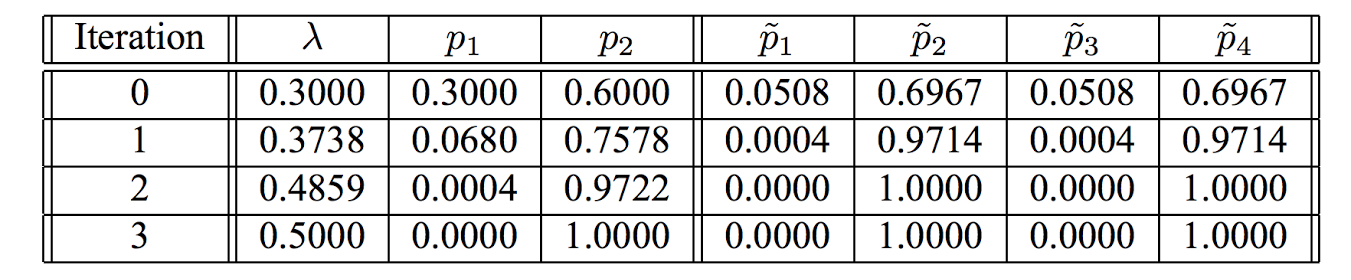
\includegraphics[width=\linewidth]{em-good.png}
	\caption{The coin example for $\mathbf{y} = \{HHH, TTT, HHH, TTT\}$. The solution that EM reaches is intuitively correct: the coin-tosser has two coins, one which always shows up heads, the other which always shows tails, and is picking between them with equal probability $(\lambda = 0.5)$. The posterior probabilities $\tilde{p}_i$ show that we are certain on coin 1 (tail-biased) generated $y_2$ and $y_4$, whereas coin 2 generated $y_1$ and $y_3$.} 
	\label{em-good}
	\centering
\end{figure}

\begin{figure}
	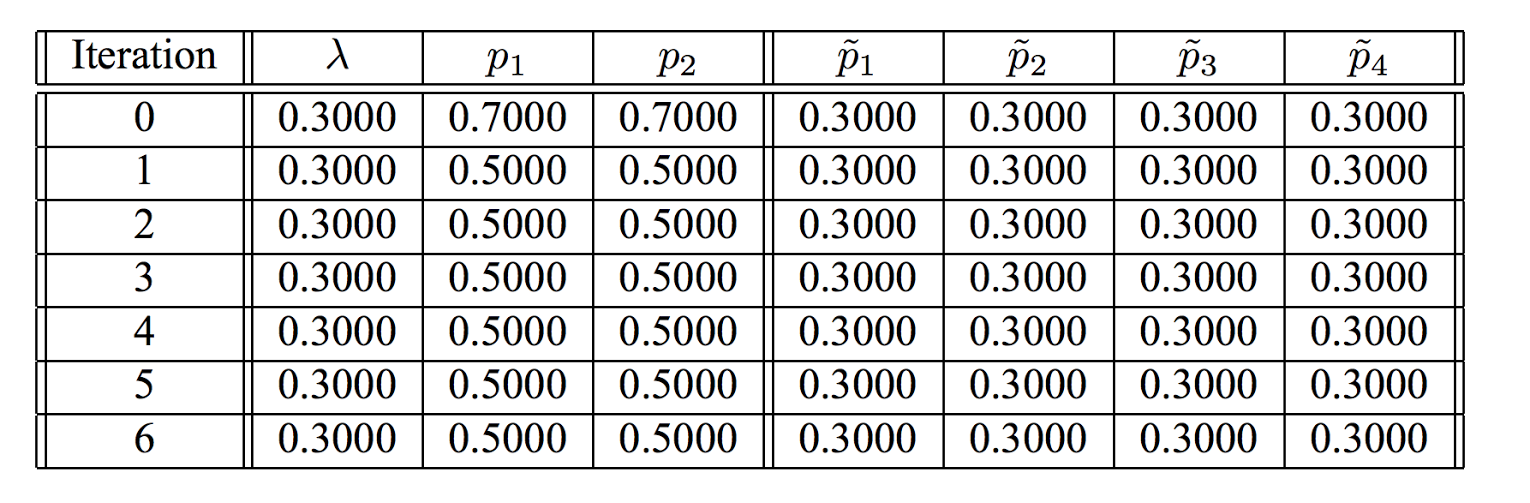
\includegraphics[width=\linewidth]{em-bad.png}
	\caption{The coin example for $\mathbf{y} = \{HHH, TTT, HHH, TTT\}$, with $p_1$ and $p_2$ initialized to the same value. EM is stuck at a saddle point. }
	\label{em-bad}
	\centering
	\setfloatalignment{c}% forces caption to be center-aligned
\end{figure}

On final note, when $y$ is hidden, it is also likely that we do not have previous knowledge of the dimension of the alphabet space, or $|\mathcal{Y}|$, such as the number of topics in the Topic Model. The dimension value can be configured by optimizing the model on a development corpus.

\section{Topic Model}\label{sec:topic-model}

\begin{figure}
	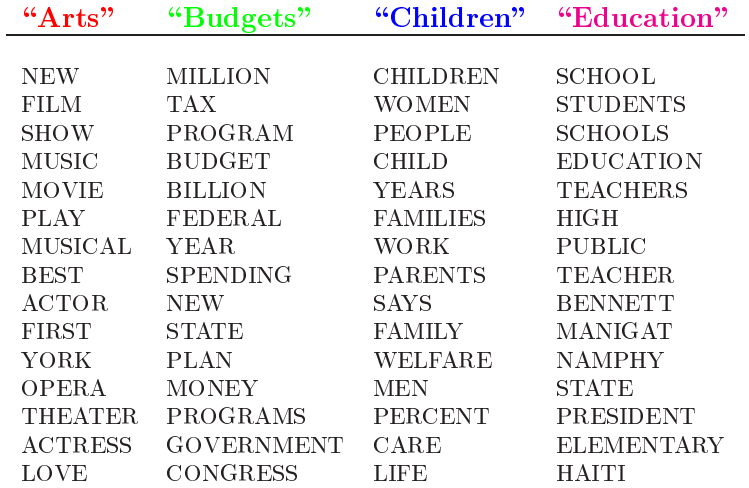
\includegraphics[width=50ex]{topic-model-table.png}
	\caption{For each given topic, some words are more likely to appear than others.}
	\centering
\end{figure}

\begin{comment}
\begin{table}[h]
	\centering
	\caption{For each given topic, some words are more likely to appear than others}
	\begin{tabular}{cccc}
		\toprule
		"Art" & "Budget" & "Children" & "Education"  \\
		\midrule
		new & money & care & state \\
		film & congress & percent & president \\
		show & & family & schools \\
		& & welfare & Haiti \\
		\bottomrule \\
	\end{tabular}
\end{table}
\end{comment}

\subsection{Introduction to Topic Model} 
In this section, we will briefly introduce Topic Model. Consider a simple unigram model where the probability of a word $w_i$ is given by $p(w_i)=\theta_i$. We will also model the topic $z$ such that $z\in\mathcal{Z}$ and $|\mathcal{Z}=k|$, where $\mathcal{Z}$ is our universe of topics and the dimension $k$ is treated as a hyperparameter. There will be a distribution over topics $z$ given by $\theta_z$, where $\sum_{z\in\mathcal{Z}}\theta_z=1$. Furthermore, each word in the document will be generated from the multinomial distribution $p(w_i|z) = \theta_{w_i|z}$, where $\sum_{i=1}^{|V|}{\theta_{w_i|z}=1}$. Consider the following steps to generate a document $\\$


\begin{enumerate}
	\item Sample a topic $z$, such that $z \sim \theta_z$
	\item \textbf{For} $i=1$ to $N$: \\  \indent\hspace{20pt} Sample words $w_i$ given the topic $z$, such that $w_i \sim \theta_{w_i|z}\\$
\end{enumerate}

\noindent Then, the likelihood of the document $d$ of size $N$ can be expressed as
\begin{align*}
p(d|\bm{\uptheta}) = \sum_{z\in\mathcal{Z}}\theta_z\prod_{i=1}^{N}\theta_{w_i|z}
\end{align*}
However, this model is problematic because it assumes that the whole document comes from a single topic. To attain a more flexible model, we should allow multiple topics in the same document. This motivation leads us to the \textit{mixture model} where each word can select its own topic. 

In this alternative approach, we setup a new model where each word $w_i$ is sampled from each corresponding topic $z_i$. In other words, every word is a mixture of topics. The sampling procedure will now become


\begin{enumerate}
	\item \textbf{For} $i=1$ to $N$: \\
	\indent\hspace{20pt} 
	Sample a topic $z_i$, such that $z_i \sim \theta_{z|d}$ \\
	\indent\hspace{20pt} 
	Sample a word $w_i$ given the topic $z_i$, such that $w_i \sim \theta_{w_i|z}\\$
\end{enumerate}

\noindent The likelihood for the new model is
\begin{align*}
p_(d|\bm{\uptheta})=\prod_{i=1}^{N}\sum_{z\in\mathcal{Z}}\theta_{z|d}\theta_{w_i|z}
\end{align*}

The distribution over the topics is unique for each document, represented by $\theta_{z|d}$. Across all documents, the word conditional on a given topic is sampled from a single "shared" distribution, represented by $\theta_{w|z}$. It is easy to see that if both the words and topics are fully observed, we can derive the MLE parameters by looking at the empirical distributions
\begin{align*}
\hat{\theta}_{w_i|z} &= \dfrac{\text{count}(w_i,z)}{\text{count}(z)} \\*
\hat{\theta}_{z|d} &= \dfrac{\text{count}(z)}{N}
\end{align*}

In application, however, topic information are not given out in the training data and the problem should be treated as a Hidden Variable Model. We leave it to the readers to think about how the EM algorithm can be applied to solve this specific unigram topic model. 

\end{document}
